% Options for packages loaded elsewhere
\PassOptionsToPackage{unicode}{hyperref}
\PassOptionsToPackage{hyphens}{url}
\PassOptionsToPackage{dvipsnames,svgnames,x11names}{xcolor}
%
\documentclass[
  letterpaper,
  DIV=11,
  numbers=noendperiod]{scrartcl}

\usepackage{amsmath,amssymb}
\usepackage{iftex}
\ifPDFTeX
  \usepackage[T1]{fontenc}
  \usepackage[utf8]{inputenc}
  \usepackage{textcomp} % provide euro and other symbols
\else % if luatex or xetex
  \usepackage{unicode-math}
  \defaultfontfeatures{Scale=MatchLowercase}
  \defaultfontfeatures[\rmfamily]{Ligatures=TeX,Scale=1}
\fi
\usepackage{lmodern}
\ifPDFTeX\else  
    % xetex/luatex font selection
\fi
% Use upquote if available, for straight quotes in verbatim environments
\IfFileExists{upquote.sty}{\usepackage{upquote}}{}
\IfFileExists{microtype.sty}{% use microtype if available
  \usepackage[]{microtype}
  \UseMicrotypeSet[protrusion]{basicmath} % disable protrusion for tt fonts
}{}
\makeatletter
\@ifundefined{KOMAClassName}{% if non-KOMA class
  \IfFileExists{parskip.sty}{%
    \usepackage{parskip}
  }{% else
    \setlength{\parindent}{0pt}
    \setlength{\parskip}{6pt plus 2pt minus 1pt}}
}{% if KOMA class
  \KOMAoptions{parskip=half}}
\makeatother
\usepackage{xcolor}
\setlength{\emergencystretch}{3em} % prevent overfull lines
\setcounter{secnumdepth}{-\maxdimen} % remove section numbering
% Make \paragraph and \subparagraph free-standing
\makeatletter
\ifx\paragraph\undefined\else
  \let\oldparagraph\paragraph
  \renewcommand{\paragraph}{
    \@ifstar
      \xxxParagraphStar
      \xxxParagraphNoStar
  }
  \newcommand{\xxxParagraphStar}[1]{\oldparagraph*{#1}\mbox{}}
  \newcommand{\xxxParagraphNoStar}[1]{\oldparagraph{#1}\mbox{}}
\fi
\ifx\subparagraph\undefined\else
  \let\oldsubparagraph\subparagraph
  \renewcommand{\subparagraph}{
    \@ifstar
      \xxxSubParagraphStar
      \xxxSubParagraphNoStar
  }
  \newcommand{\xxxSubParagraphStar}[1]{\oldsubparagraph*{#1}\mbox{}}
  \newcommand{\xxxSubParagraphNoStar}[1]{\oldsubparagraph{#1}\mbox{}}
\fi
\makeatother


\providecommand{\tightlist}{%
  \setlength{\itemsep}{0pt}\setlength{\parskip}{0pt}}\usepackage{longtable,booktabs,array}
\usepackage{calc} % for calculating minipage widths
% Correct order of tables after \paragraph or \subparagraph
\usepackage{etoolbox}
\makeatletter
\patchcmd\longtable{\par}{\if@noskipsec\mbox{}\fi\par}{}{}
\makeatother
% Allow footnotes in longtable head/foot
\IfFileExists{footnotehyper.sty}{\usepackage{footnotehyper}}{\usepackage{footnote}}
\makesavenoteenv{longtable}
\usepackage{graphicx}
\makeatletter
\def\maxwidth{\ifdim\Gin@nat@width>\linewidth\linewidth\else\Gin@nat@width\fi}
\def\maxheight{\ifdim\Gin@nat@height>\textheight\textheight\else\Gin@nat@height\fi}
\makeatother
% Scale images if necessary, so that they will not overflow the page
% margins by default, and it is still possible to overwrite the defaults
% using explicit options in \includegraphics[width, height, ...]{}
\setkeys{Gin}{width=\maxwidth,height=\maxheight,keepaspectratio}
% Set default figure placement to htbp
\makeatletter
\def\fps@figure{htbp}
\makeatother

\KOMAoption{captions}{tableheading}
\makeatletter
\@ifpackageloaded{caption}{}{\usepackage{caption}}
\AtBeginDocument{%
\ifdefined\contentsname
  \renewcommand*\contentsname{Table of contents}
\else
  \newcommand\contentsname{Table of contents}
\fi
\ifdefined\listfigurename
  \renewcommand*\listfigurename{List of Figures}
\else
  \newcommand\listfigurename{List of Figures}
\fi
\ifdefined\listtablename
  \renewcommand*\listtablename{List of Tables}
\else
  \newcommand\listtablename{List of Tables}
\fi
\ifdefined\figurename
  \renewcommand*\figurename{Figure}
\else
  \newcommand\figurename{Figure}
\fi
\ifdefined\tablename
  \renewcommand*\tablename{Table}
\else
  \newcommand\tablename{Table}
\fi
}
\@ifpackageloaded{float}{}{\usepackage{float}}
\floatstyle{ruled}
\@ifundefined{c@chapter}{\newfloat{codelisting}{h}{lop}}{\newfloat{codelisting}{h}{lop}[chapter]}
\floatname{codelisting}{Listing}
\newcommand*\listoflistings{\listof{codelisting}{List of Listings}}
\makeatother
\makeatletter
\makeatother
\makeatletter
\@ifpackageloaded{caption}{}{\usepackage{caption}}
\@ifpackageloaded{subcaption}{}{\usepackage{subcaption}}
\makeatother

\ifLuaTeX
  \usepackage{selnolig}  % disable illegal ligatures
\fi
\usepackage{bookmark}

\IfFileExists{xurl.sty}{\usepackage{xurl}}{} % add URL line breaks if available
\urlstyle{same} % disable monospaced font for URLs
\hypersetup{
  pdftitle={Reproduction of 'Sexism and the far-right vote: The Individual dynamics of gender backlash by Eva Anduiza \& Guillem Rico},
  pdfauthor={Jenna Brooks},
  colorlinks=true,
  linkcolor={blue},
  filecolor={Maroon},
  citecolor={Blue},
  urlcolor={Blue},
  pdfcreator={LaTeX via pandoc}}


\title{Reproduction of 'Sexism and the far-right vote: The Individual
dynamics of gender backlash by Eva Anduiza \& Guillem Rico}
\author{Jenna Brooks}
\date{}

\begin{document}
\maketitle


\begin{verbatim}
Loading required package: ggplot2
\end{verbatim}

\begin{verbatim}

Please cite as: 
\end{verbatim}

\begin{verbatim}
 Hlavac, Marek (2022). stargazer: Well-Formatted Regression and Summary Statistics Tables.
\end{verbatim}

\begin{verbatim}
 R package version 5.2.3. https://CRAN.R-project.org/package=stargazer 
\end{verbatim}

\begin{verbatim}
Loading required package: grid
\end{verbatim}

\begin{verbatim}
Loading required package: Matrix
\end{verbatim}

\begin{verbatim}
Loading required package: survival
\end{verbatim}

\begin{verbatim}

Attaching package: 'survey'
\end{verbatim}

\begin{verbatim}
The following object is masked from 'package:graphics':

    dotchart
\end{verbatim}

\begin{verbatim}

Attaching package: 'dplyr'
\end{verbatim}

\begin{verbatim}
The following objects are masked from 'package:stats':

    filter, lag
\end{verbatim}

\begin{verbatim}
The following objects are masked from 'package:base':

    intersect, setdiff, setequal, union
\end{verbatim}

\begin{verbatim}
corrplot 0.95 loaded
\end{verbatim}

\section{Reproduction of ``Sexism and the far-right vote: The individual
dynamics of gender
backlash''}\label{reproduction-of-sexism-and-the-far-right-vote-the-individual-dynamics-of-gender-backlash}

Authors: Eva Anduiza \& Guillem Rico

This paper examines how sexism has played a role the electoral rise of
the far-right party, Vox, in Spain. Anduiza and Rico () argue that
having sexist beliefs is one of the most influential attitudinal
predictors of voting for the far-right party Vox.

\subsection{Original Study}\label{original-study}

\subsubsection{Data}\label{data}

Using panel data from Spain, collected before, during and after
prominent feminist protests in 2018 and 2019, the authors assess
individual changes in measures of sexism occurring in various contexts
of feminist movement and the surge of far right support.

The data utilized in this study is drawn from the Spanish Political
Attitudes dataset (Hernández Pérez et al., 2021), a longitudinal online
panel survey conducted annually. The survey uses a quota sampling method
to ensure a representative sample of the Spanish adult population aged
18 to 56, with quotas based on gender, age, educational background,
geographic region, and municipality size. The unit of analysis is
individual voters in Spain.

Observational independence could be questioned in this data set due to
the longitudinal design (repeated observations) and the geographic
clustering of like-minded voters in specific regions, as well as
demographic factors such as age, gender, and education.

This study specifically examines the four survey waves conducted between
2017 and 2020, as these waves include the modern sexism battery, which
is central to the analysis. Key to the analysis was the collection of
the first wave of data before the first massive feminist movement and
the second wave before the rise of the far-right party Vox.

\subsubsection{Dependent Variable: Vote for
Vox}\label{dependent-variable-vote-for-vox}

The dependent variable in this study is binary -- the intention to vote
for Vox, coded as 1, with all other responses, including non-responses
and nonvoters, coded as 0. This measure is based on respondents' answers
to the question, ``Which party would you vote for if the general
elections were tomorrow?'' The authors chose to analyze voting intention
rather than past voting behavior to capture respondents' support for Vox
at the exact moment of their interview. Given that Vox did not gain
significant traction until late 2018, the analysis of voter intention is
restricted to the 2019 and 2020 waves of the survey.

The dataset initially comprised 7,850 observations for vote intentions.
However, after filtering the data to include only the years 2019 and
2020, the total number of observations was reduced to 3,491. Within this
subset, 258 observations (approximately 7.39\%) correspond to votes for
Vox, the dependent variable of interest, while the remaining 3,233
observations (approximately 92.61\%) represent votes for other political
parties in Spain.

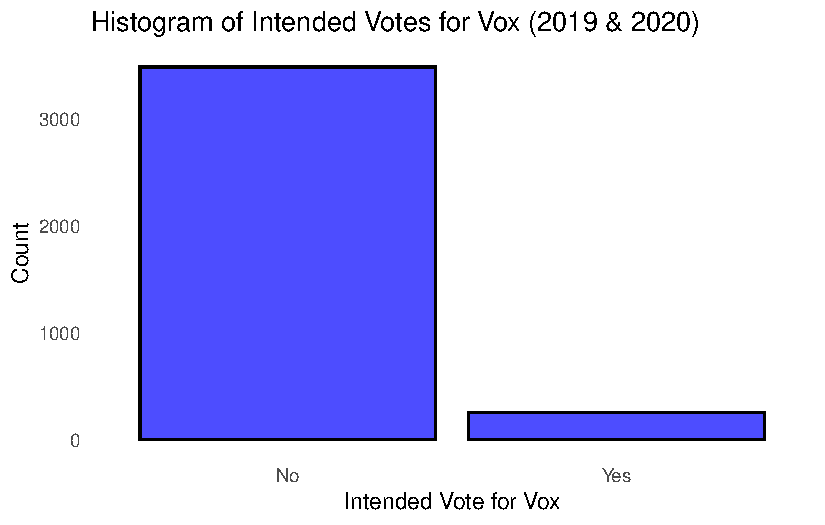
\includegraphics{reprod_sexism_files/figure-pdf/unnamed-chunk-3-1.pdf}

\begin{verbatim}

   0    1 
3491  258 
\end{verbatim}

The histogram above, which depicts intended votes for Vox (coded as 1
for ``Yes'' and 0 for ``No''), continues to show a binary distribution,
with a significantly higher frequency of 0s (non-Vox voters) compared to
1s (Vox voters). This refined approach provides a more precise
assessment of Vox's appeal during its period of rising popularity.

\textbf{Plot and Distribution:}

The dataset comprises a total of 7,850 observations for vote intentions,
of which 299 instances (approximately 3.81\%) correspond to votes for
Vox, the dependent variable of interest, while the remaining 7,551
observations (approximately 96.19\%) represent votes for other political
parties in Spain. The histogram above, which represents the intended
vote for Vox (coded 1 for Yes, 0 for No), shows a binary distribution,
with a higher frequency of 0s (non-Vox voters) compared to 1s (Vox
voters).

\subsubsection{Data Cleaning and Missing
Data}\label{data-cleaning-and-missing-data}

\begin{itemize}
\item
  Income (missing values imputed from other waves)
\item
  na.rm = True a lot for NAs
\item
  The (.=.) part ensures that missing values (.) in the original
  variables are preserved in the new variables. (under modern sexism
  scale)
\end{itemize}

\begin{verbatim}
[1] TRUE
\end{verbatim}

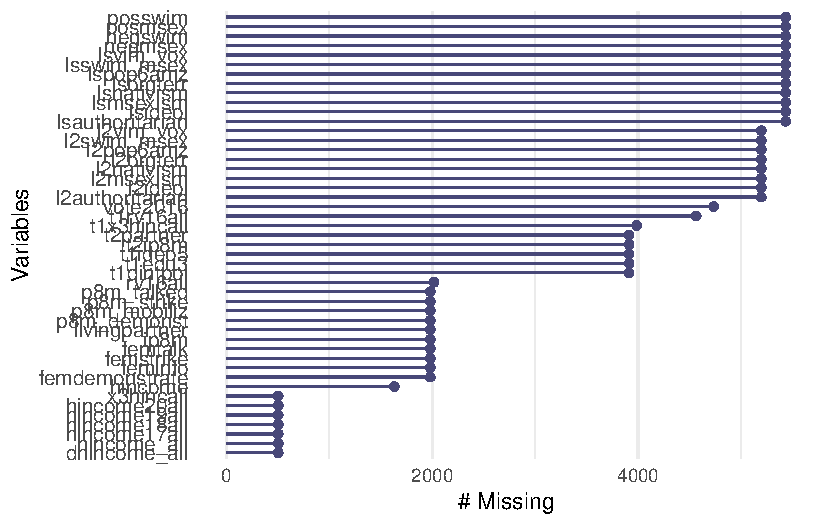
\includegraphics{reprod_sexism_files/figure-pdf/unnamed-chunk-4-1.pdf}

\subsubsection{Other Attitudinal
Factors}\label{other-attitudinal-factors}

Anduiza and Rico include a set of control variables to account for
potential confounding factors leading to a vote for the far right. These
factors included \textbf{General ideological identification}, measured
on an 11-point left--right scale; \textbf{Authoritarianism}, assessed
using a 4-item battery based on childrearing values (Feldman and Stenner
1997); \textbf{Nativism}, which evaluates attitudes toward the economic
and cultural impacts of migration; \textbf{Populist attitudes},
operationalized using the framework developed by Akkerman, Mudde, and
Zaslove (2014); and \textbf{Territorial preferences}, where higher
values indicate stronger support for decentralization. Additionally, the
model controlled for sex, age, education (middle school or less, high
school/vocational training, college), whether the respondent lives with
a partner, household income (a scale with 12 intervals), and a 4-point
measure of interest in politics. With the exception of age (in years),
all variables were recoded to run from zero to one.

\subsubsection{Model: Table 1}\label{model-table-1}

My analysis will be replicating Table 1 ``Predictors of Intention to
Vote for Vox in 2019 and 2020'' (pg.487). The authors hope to achieve a
descriptive analysis in this paper, assessing how sexist attitudes,
alongside other factors typically associated with voting for the
far-right, are associated with support for Vox.

Table 1 displays the the estimates of \textbf{two cross-sectional logit
models} of intended vote for the 2019 and 2020 waves, respectively:

\[
vox_{it} = sexism_{it} + other\_attitudes_{it} + controls_{it}
\]

where \(i\) indexes individuals and \(t\) as time (wave);
\(other\_attitudes_{it}\) encompasses measures of ideology,
authoritarianism, nativism, territorial preferences, and populism; and
the controls include sex, age, education, income, living with a partner,
and interest in politics.

\begin{verbatim}

Reproduction of Predictors of Intention to Vote for Vox in 2019 and 2020
==============================================
                      Dependent variable:     
                  ----------------------------
                              vim             
                       2019          2020     
                       (1)            (2)     
----------------------------------------------
female                0.118         -0.145    
                     (0.277)        (0.220)   
                                              
age                   0.004         -0.009    
                     (0.016)        (0.010)   
                                              
factor(edu3)2         -0.716         0.198    
                     (0.442)        (0.286)   
                                              
factor(edu3)3         -0.075         0.080    
                     (0.300)        (0.256)   
                                              
dhincome_all          -0.529        -0.061    
                     (0.575)        (0.446)   
                                              
livingpartner         0.192          0.018    
                     (0.301)        (0.231)   
                                              
intpol                0.634         0.915**   
                     (0.478)        (0.364)   
                                              
authoritarian         -0.499         0.136    
                     (0.540)        (0.408)   
                                              
ideol                5.497***      4.965***   
                     (0.729)        (0.587)   
                                              
nativism             2.646***      2.280***   
                     (0.655)        (0.564)   
                                              
orgterr              -1.314**      -1.905***  
                     (0.528)        (0.398)   
                                              
pop6amz               0.894         1.418**   
                     (0.741)        (0.625)   
                                              
msexism              4.159***      2.983***   
                     (0.749)        (0.583)   
                                              
Constant            -9.712***      -8.419***  
                     (1.189)        (0.829)   
                                              
----------------------------------------------
Observations          1,651          1,972    
Log Likelihood       -230.096      -360.017   
Akaike Inf. Crit.    488.192        748.034   
==============================================
Note:              *p<0.1; **p<0.05; ***p<0.01

Reproduction of Predictors of Intention to Vote for Vox in 2019 and 2020
=
n
-
\end{verbatim}

\begin{figure}[H]

{\centering 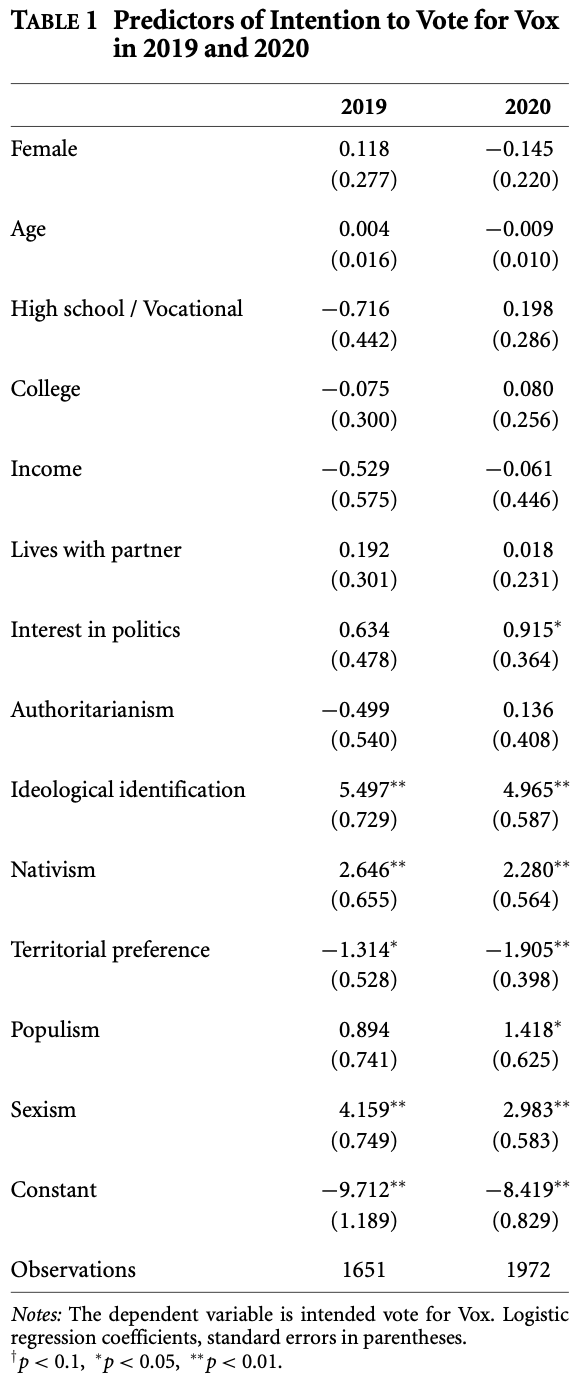
\includegraphics{images/Screenshot 2025-03-04 at 2.04.58 PM.png}

}

\caption{\textbf{Author's Table 1 reflects the same results as my table
above.}}

\end{figure}%

The models indicate that the effects of the attitudinal variables align
with the authors' expectations: support for Vox was positively
associated with right-wing ideology, sexism, nativism, and populist
attitudes (with the latter reaching statistical significance only in
2020), while it is negatively associated with attitudes favoring
decentralization. Among these factors, modern sexism has the
second-largest impact, surpassed only by ideological orientation. When
holding all other variables constant at their observed values,
individuals in the 95th percentile of the sexism scale are 8.6
percentage points (in 2019) and 9.9 percentage points (in 2020) more
likely to express an intention to vote for Vox compared to those in the
5th percentile. This reiterates the authors' argument that sexism plays
a prominent role in an intention to vote for the far-right party, Vox.

\section{Additional Models}\label{additional-models}

\subsubsection{Different Link Functions}\label{different-link-functions}

In my analysis, I chose to focus specifically on the 2020 data from
Table 1 to simplify the comparison of the models. I fit two additional
models to the original -- a probit and a cloglog model on the same
dependent variable and covariates.

My primary aim was to investigate whether altering the link function
from logit to probit or cloglog resulted in any measurable differences
in performance. This exploration was driven by an interest in
understanding the comparative behavior of probit, logit, and cloglog
models when applied to binary data, particularly in terms of their
predictive accuracy and suitability for the dataset.

Specifically, I was interested in the cloglog to anlayze instances of
rare events in binary data. Given the low frequency of ``1''s in the
dependent variable (a vote for Vox), I hypothesized that rare events
might be a significant feature of my dataset. By incorporating the
cloglog, I aimed to ensure that the analysis could effectively capture
and model the infrequent occurrences of the event of interest, providing
a more robust evaluation of the data. \#\#\#\# Probit and ClogLog:

\begin{verbatim}

Reproduction of Predictors of Intention to Vote for Vox in 2020
=======================================================
                           Dependent variable:         
                  -------------------------------------
                                   vim                 
                   logistic    probit    glm: binomial 
                                         link = cloglog
                  2020 Logit 2020 Probit  2020 Cloglog 
                     (1)         (2)          (3)      
-------------------------------------------------------
female              -0.145     -0.051        -0.149    
                   (0.220)     (0.111)      (0.186)    
                                                       
age                 -0.009     -0.007        -0.009    
                   (0.010)     (0.005)      (0.009)    
                                                       
factor(edu3)2       0.198       0.119        0.065     
                   (0.286)     (0.144)      (0.250)    
                                                       
factor(edu3)3       0.080       0.005        0.149     
                   (0.256)     (0.130)      (0.216)    
                                                       
dhincome_all        -0.061     -0.013        -0.115    
                   (0.446)     (0.228)      (0.374)    
                                                       
livingpartner       0.018      0.0004        -0.041    
                   (0.231)     (0.116)      (0.198)    
                                                       
intpol             0.915**    0.534***      0.839***   
                   (0.364)     (0.188)      (0.302)    
                                                       
authoritarian       0.136       0.151        0.073     
                   (0.408)     (0.206)      (0.349)    
                                                       
ideol              4.965***   2.363***      4.142***   
                   (0.587)     (0.303)      (0.470)    
                                                       
nativism           2.280***   1.363***      1.843***   
                   (0.564)     (0.292)      (0.466)    
                                                       
orgterr           -1.905***   -0.879***    -1.712***   
                   (0.398)     (0.194)      (0.353)    
                                                       
pop6amz            1.418**     0.783**      1.297**    
                   (0.625)     (0.321)      (0.527)    
                                                       
msexism            2.983***   1.588***      2.219***   
                   (0.583)     (0.305)      (0.482)    
                                                       
Constant          -8.419***   -4.483***    -7.240***   
                   (0.829)     (0.416)      (0.684)    
                                                       
-------------------------------------------------------
Observations        1,972       1,972        1,972     
Log Likelihood     -360.017   -363.769      -361.747   
Akaike Inf. Crit.  748.034     755.537      751.494    
=======================================================
Note:                       *p<0.1; **p<0.05; ***p<0.01
\end{verbatim}

\subparagraph{In Sample Comparison of
Models}\label{in-sample-comparison-of-models}

As shown in the table above, the original logit model outperforms both
the probit and cloglog models. The logit model has the lowest AIC value,
which suggests better in-sample performance. The cloglog model ranks
second in terms of AIC, while the probit model ranks third for in-
sample performance, however the relative difference in performance is
negligible. Furthermore, the logit model achieves the highest
log-likelihood value, further confirming its better performance. These
results indicate that the original logit model is the most effective
among the three for this dataset.

\subparagraph{Out of Sample Performance: 10-Fold Cross
Validation}\label{out-of-sample-performance-10-fold-cross-validation}

There is evidence of perfect separation in my dataset.

\begin{verbatim}
Loading required package: lattice
\end{verbatim}

\begin{verbatim}

Attaching package: 'caret'
\end{verbatim}

\begin{verbatim}
The following object is masked from 'package:survival':

    cluster
\end{verbatim}

\begin{verbatim}
    Model MSE
1   Logit  NA
2  Probit  NA
3 Cloglog  NA
\end{verbatim}

\subsection{2. Multiplicative
relationship}\label{multiplicative-relationship}

I decided to look at the multiplicative relationship between nativism
and modern sexism because these beliefs tend to coincide as predictors
of rightwing support. If someone is nativist but not high in msexism,
they might support another party, however with both they are likely to
support far right.

include another predictor variable that author didn't use.

try gender * msexism - I think men are more likely to be sexist lol

\begin{verbatim}

Reproduction of Predictors of Intention to Vote for Vox in 2019 and 2020
====================================================================================================
                                                 Dependent variable:                                
                  ----------------------------------------------------------------------------------
                                                         vim                                        
                  2019 Logit 2019 Multiplicative Nativism * Sexism 2020 Logit 2020 Nativism * Sexism
                     (1)                      (2)                     (3)              (4)          
----------------------------------------------------------------------------------------------------
female              0.118                    0.121                   -0.145           -0.137        
                   (0.277)                  (0.277)                 (0.220)          (0.219)        
                                                                                                    
age                 0.004                    0.004                   -0.009           -0.010        
                   (0.016)                  (0.016)                 (0.010)          (0.010)        
                                                                                                    
factor(edu3)2       -0.716                  -0.708                   0.198            0.202         
                   (0.442)                  (0.441)                 (0.286)          (0.285)        
                                                                                                    
factor(edu3)3       -0.075                  -0.076                   0.080            0.086         
                   (0.300)                  (0.299)                 (0.256)          (0.255)        
                                                                                                    
dhincome_all        -0.529                  -0.546                   -0.061           -0.061        
                   (0.575)                  (0.575)                 (0.446)          (0.445)        
                                                                                                    
livingpartner       0.192                    0.195                   0.018            0.025         
                   (0.301)                  (0.300)                 (0.231)          (0.230)        
                                                                                                    
intpol              0.634                    0.651                  0.915**          0.930**        
                   (0.478)                  (0.478)                 (0.364)          (0.364)        
                                                                                                    
authoritarian       -0.499                  -0.513                   0.136            0.149         
                   (0.540)                  (0.540)                 (0.408)          (0.408)        
                                                                                                    
ideol              5.497***                5.485***                 4.965***         4.911***       
                   (0.729)                  (0.731)                 (0.587)          (0.587)        
                                                                                                    
nativism           2.646***                 3.572*                  2.280***         4.047***       
                   (0.655)                  (1.933)                 (0.564)          (1.541)        
                                                                                                    
orgterr            -1.314**                -1.321**                -1.905***        -1.907***       
                   (0.528)                  (0.528)                 (0.398)          (0.397)        
                                                                                                    
pop6amz             0.894                    0.897                  1.418**          1.410**        
                   (0.741)                  (0.741)                 (0.625)          (0.622)        
                                                                                                    
msexism            4.159***                 5.388**                 2.983***         5.178***       
                   (0.749)                  (2.533)                 (0.583)          (1.884)        
                                                                                                    
nativism:msexism                            -1.699                                    -3.214        
                                            (3.328)                                  (2.595)        
                                                                                                    
Constant          -9.712***               -10.359***               -8.419***        -9.571***       
                   (1.189)                  (1.752)                 (0.829)          (1.266)        
                                                                                                    
----------------------------------------------------------------------------------------------------
Observations        1,651                    1,651                   1,972            1,972         
Log Likelihood     -230.096                -229.966                 -360.017         -359.248       
Akaike Inf. Crit.  488.192                  489.932                 748.034          748.496        
====================================================================================================
Note:                                                                    *p<0.1; **p<0.05; ***p<0.01
\end{verbatim}

```

\section{\texorpdfstring{\texttt{\{r\}\ \#\ \#\ library(lmtest)\ \#\ lrtest(t1m1,\ t1simp)\ \#}}{\{r\} \# \# library(lmtest) \# lrtest(t1m1, t1simp) \#}}\label{r-librarylmtest-lrtestt1m1-t1simp}

\subsection{A correlation matrix for the DV and IVs that the original
authors included in the model you are
replicating}\label{a-correlation-matrix-for-the-dv-and-ivs-that-the-original-authors-included-in-the-model-you-are-replicating}

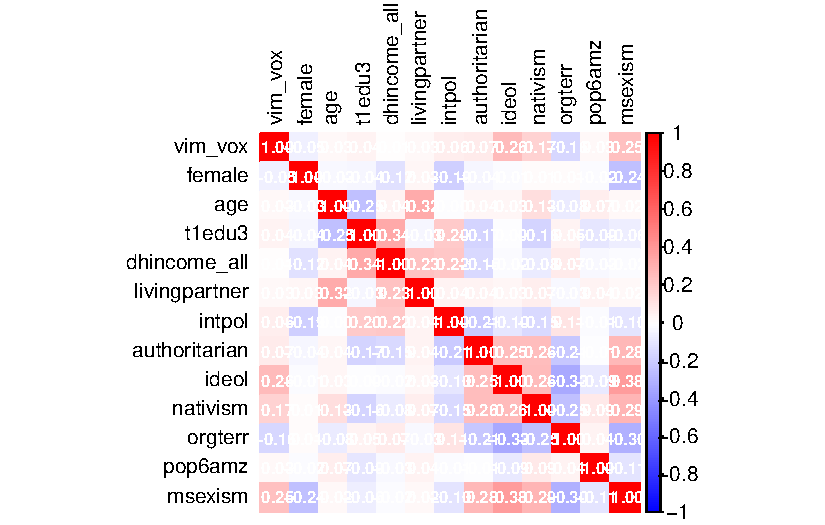
\includegraphics{reprod_sexism_files/figure-pdf/unnamed-chunk-9-1.pdf}

\subsection{Cross Validation}\label{cross-validation}

\subsection{Interpretive Exercise (Scenarios) for the better
model}\label{interpretive-exercise-scenarios-for-the-better-model}

\begin{itemize}
\item
  explain why you chose the values you did?
\item
  Women - more likely to vote for vox? or less? M vs.~F?
\item
\end{itemize}

\section{Limitations}\label{limitations}

The authors mention ``We, thus, cannot rule out that Vox voters'
opinions on women's discrimination are actually a consequence, rather
than a cause, of their partisan preferences.'' (pg. 486)

Evaluate both models and come to a conclusion based on the

Use cross validation to get out of sample error for OG and your new
model --\textgreater{} based on what I did, my new model doesn't really
add anything to the outcome

not trying to overturn the author's original findings. or find a better
model

\section{Citations:}\label{citations}

Swim et al (1995) Stargazer Library

\section{AI Appendix Statement (update
this):}\label{ai-appendix-statement-update-this}

\begin{itemize}
\item
  I used ChatGPT LLM/AI tool in this assignment.
\item
  I used it to help write the code for the plots. ~
\item
  I found it helpful in getting the results I was looking for and
  understanding the concept of a correlation matrix. Also helped with
  converting DTA to CSV
\item
  Link:
  \url{https://chatgpt.com/share/67af9007-561c-800f-9f0f-367b9f306c7e}
\end{itemize}

Link2:
\url{https://chatgpt.com/share/67af908c-6de0-800f-aca5-1a1cdb82be69}

Link3: \url{https://chatgpt.com/c/67c76a1c-e874-800d-84f0-e5ddc106c044}

Link4:\\




\end{document}
